\bta{波粒二象性}


\begin{enumerate}
	%\renewcommand{\labelenumi}{\arabic{enumi}.}
	% A(\Alph) a(\alph) I(\Roman) i(\roman) 1(\arabic)
	%设定全局标号series=example	%引用全局变量resume=example
	%[topsep=-0.3em,parsep=-0.3em,itemsep=-0.3em,partopsep=-0.3em]
	%可使用leftmargin调整列表环境左边的空白长度 [leftmargin=0em]
	\item
\exwhere{$ 2015 $ 年上海卷}
 用很弱的光做单缝衍射实验,改变曝光时间,在胶片上出现的图像如图所示,
该实验表明 \xzanswer{C} 
% TODO: \usepackage{graphicx} required
\begin{figure}[h!]
	\centering
	\begin{subfigure}{0.22\linewidth}
		\centering
		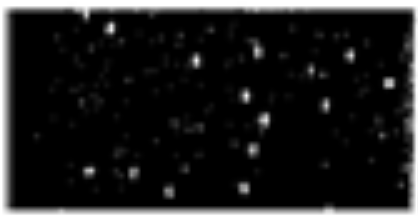
\includegraphics[width=0.85\linewidth]{picture/screenshot076}
		\caption{时间较短}\label{}
	\end{subfigure}
	\begin{subfigure}{0.22\linewidth}
		\centering
		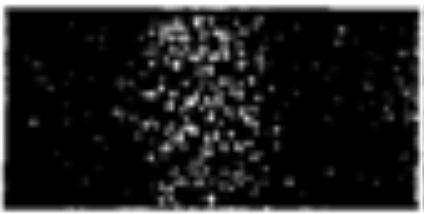
\includegraphics[width=0.85\linewidth]{picture/screenshot077}
		\caption{时间稍长}\label{}
	\end{subfigure}
	\begin{subfigure}{0.22\linewidth}
		\centering
		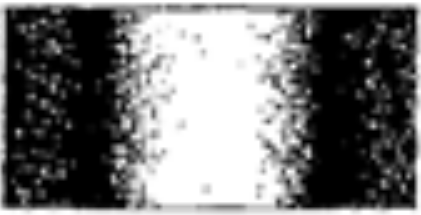
\includegraphics[width=0.85\linewidth]{picture/screenshot078}
		\caption{时间较长}\label{}
	\end{subfigure}
\end{figure}



\fourchoices
{光的本质是波}
{光的本质是粒子}
{光的能量在胶片上分布不均匀}
{光到达胶片上不同位置的概率相同}



\item 
\exwhere{$ 2011 $年上海卷}
用极微弱的可见光做双缝干涉实验,随着时间的增加,在屏上先后出现如 \subref{2011上海双缝干涉a} 、 \subref{2011上海双缝干涉b}、 \subref{2011上海双缝干涉c} 所示
的图像,则 \xzanswer{ABD}
% TODO: \usepackage{graphicx} required
\begin{figure}[h!]
	\centering
	\begin{subfigure}{0.22\linewidth}
		\centering
		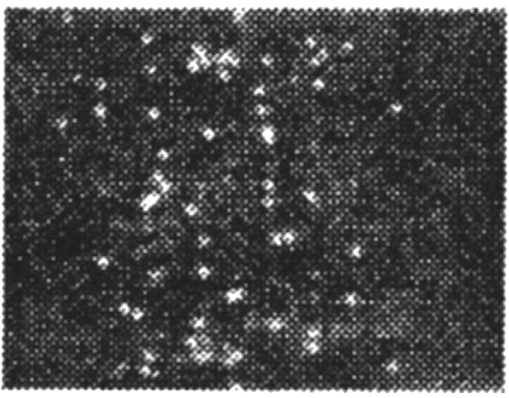
\includegraphics[width=0.85\linewidth]{picture/screenshot079}
		\caption{}\label{2011上海双缝干涉a}
	\end{subfigure}
	\begin{subfigure}{0.22\linewidth}
		\centering
		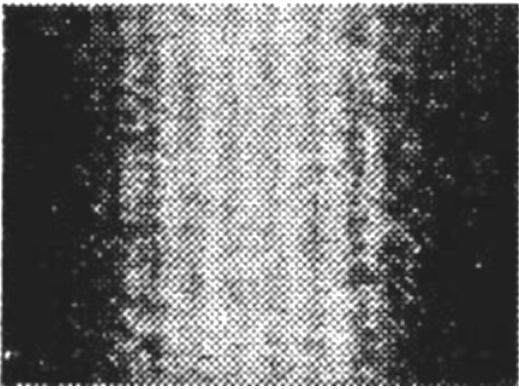
\includegraphics[width=0.85\linewidth]{picture/screenshot080}
		\caption{}\label{2011上海双缝干涉b}
	\end{subfigure}
	\begin{subfigure}{0.22\linewidth}
		\centering
		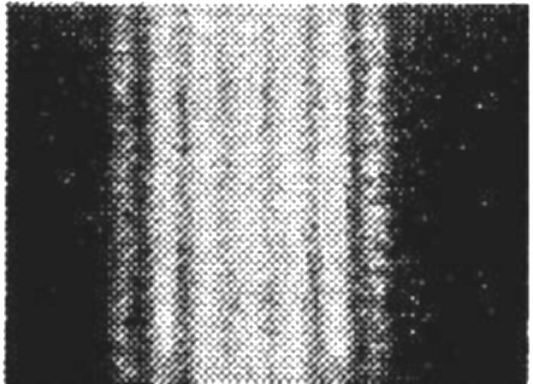
\includegraphics[width=0.85\linewidth]{picture/screenshot081}
		\caption{}\label{2011上海双缝干涉c}
	\end{subfigure}
\end{figure}
 

\fourchoices
{图像 \subref{2011上海双缝干涉a} 表明光具有粒子性}
{图像 \subref{2011上海双缝干涉c} 表明光具有波动性}
{用紫外光观察不到类似的图像}
{实验表明光是一种概率波}






	
	
	
\end{enumerate}

